\documentclass{report}

\usepackage{graphicx}
\usepackage{epstopdf}
\usepackage{bm}

\begin{document}

\chapter{Blinding with Linear Clustering Removal}
\author{Samuel Wehrli}
\date{\today}
%\maketitle

This work investigates discriminatory dimensions in face recognition algorithms. For a given discriminatory dimension, the data can be grouped into clusters (for example ethnic groups in the case of race). A blinding procedure is proposed to remove the information related to the separation of these clusters. The procedure is a linear operation in the embedding space and uses three steps

\begin{enumerate}
	\item Compute cluster centers to infer directions of discrimination 
	\item Apply SVD on the directions of discrimination to find orthonormal basis spanning the ``discriminatory subspace'' 
	\item Remove projections onto the ``discriminatory subspace'' from the embedding vectors. This results in embedding vectors are orthogonal to the directions of discrimination.
\end{enumerate} 

\noindent After outlining the method,  cluster visualization, awareness and face recognition rates are investigated before and after the blinding procedure.

\section{The math behind}

In the following we look at the discriminatory dimension of race. We work with the commonly used racial faces in-the-wild (RFW) data set which has the four ethnic labels Caucasian, African, Asian and Indian. Face recognition algorithms work with embedding spaces. They map images of persons into a vector space with dimension $N_e$. In the following I consider a VGG2 model where $N_e=128$. The mapping is optimized such that images of the same person are close to each other in the embedding space. The proposed procedure takes the empedding vectors $\bm{x}_i$ as an input ($i$ denotes the sample). Each sample corresponds to an ethnic class $k$. The goal is to remove the directions of the embedding space which separate the ethnic clusters. It is mathematically equivalent to a unitary rotation in the embedding space such that some of the features capture the cluster separation and a subsequent removal of these features. As outlined above, we define the centers of each cluster simply by averaging

\begin{equation}
\label{eq:xbar}
	\bar{\bm{x}}_k = \frac{1}{n_k}\sum_{i\in C_k}\bm{x}_i ,
\end{equation} 

\noindent where $C_k$ is the set of embedding vectors associated with cluster k and $n_k$ is the corresponding size. Following a one-vs-rest (OvR) approach, the normalized separational directions of each cluster center $\bar{\bm{x}}_k$ to the other centers is given by the vectors

\begin{equation}
\label{eq:uk}
	\bm{u}_k = \frac{\bm{v}_k}{\Vert \bm{v}_k \Vert} \quad \textrm{with} \quad \bm{v}_k = \bar{\bm{x}}_k -  \frac{1}{K-1}\sum_{k' \ne k} \bar{\bm{x}}_k,
\end{equation} 

\begin{figure}
  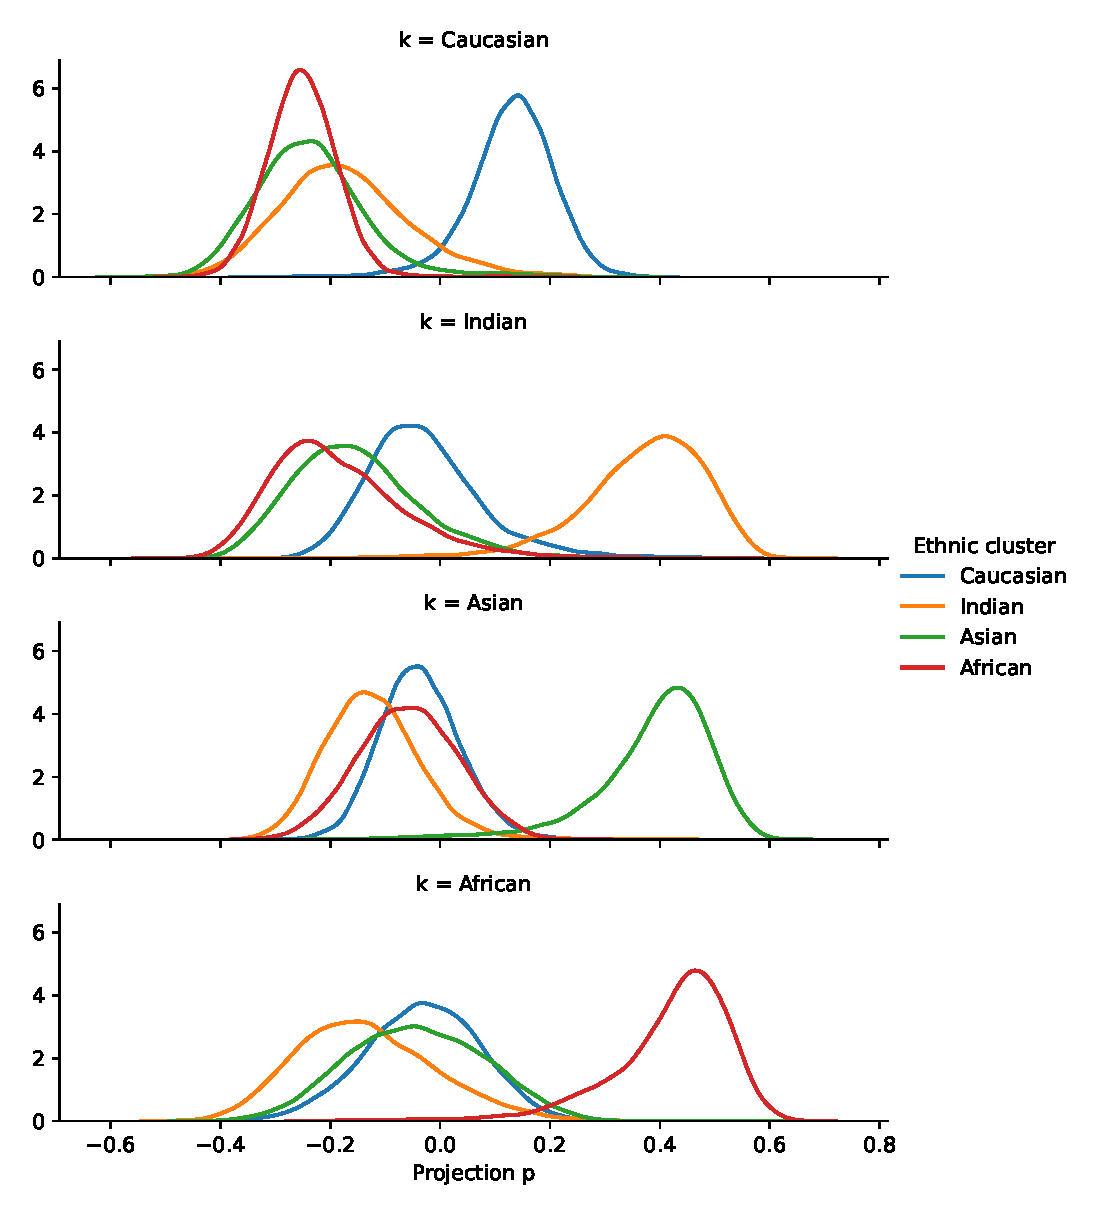
\includegraphics[width=\linewidth]{projection.eps}
  \caption{Kernel density estimation (KDE) plot of the projections  ($\bm{x}_i\cdot \bm{u}_k$). The normalized directions $\bm{u}_k$ represent the discriminatory directions.}
  \label{fig:projection}
\end{figure}

\noindent where $K$ is the number of clusters. Fig.~\ref{fig:projection} shows the projections onto the vectors $\bm{u}_k$. As it may be expected by the construction, each direction nicely separates the corresponding cluster from the others. These means, that different ethnic groups are literally located in different corners of the empedding space. By construction, the vectors $\bm{u}_k$ are not linearly independent, but span a subspace of rank $K-1$. This can by verified by applying a singular value decomposition (SVD) on the matrix $U=[\bm{u}_1\ldots \bm{u}_K]$. SVD also provides a orhtonormal basis $B=[\bm{e}_1\ldots \bm{e}_{K-1}]$ of the corresponding subspace. The final step is to remove the projections onto this subspace by

\begin{equation}
\label{eq:xb}
	\bm{x}_i^{b} = \bm{x}_i - \sum_{j=1}^{K-1} (\bm{x}_i\cdot \bm{e}_j)\,\bm{e}_j,
\end{equation} 

\noindent where $(\bm{x}_i\cdot \bm{e}_j)$ is the dot (or scalar) product.  Eq.~(\ref{eq:xb}) yields new embedding vector $\bm{x}_i^{b}$ with the same shape as the original ones. The upper index $b$ stands for \emph{blinded} inspired by the fact that some information with regard to the discriminatory dimension has been removed. Note that the new embeddings depend linearly on the original ones. 
   

\section{Awareness}

Awareness is the ability of the model to discriminate between different clusters of the discriminatory dimensions, being the ethnic label in present case. This ability obviously depends on the trained model at hand. Here I benchmark the performance to predict the ethnic labels by the \emph{aware} embeddings $x_i$ and the \emph{blinded} ones $\bm{x}_i^{b}$. Both embbedings have been split into 66.6\% training data and 33.3\% test data. The accuracy of different classifiers is shown in Tab.~\ref{tab:awareness}. Not surprisingly, linear classifiers are unable to predict the race for the blinded embeddings. Nearest neighbor approaches still work reasonably. More advanced non-linear classifiers such as neural networks perform well. The clustering displayed by the corresponding t-SNE plots in Fig.~\ref{fig:tSNE} is in line with these findings. In the blinded case, clusters can't be separated be a single straight line. However, the data still displays groups defined by ethnical labels. Interestingly, there are clear differences between the groups. Africans are grouped in the center, Caucasian encircle the cloud and Indians/Asian are scattered inbetween. 

\begin{table}
\begin{center}
\begin{tabular}{ c|c|c  }
Model & aware  & blinded  \\
\hline
Logistic regression & 96\% & 21\% \\ 
Linear SVM & 96\% & 26\% \\  
Nearest neighbor & 92\% &  57\%  \\   
5 Nearest neighbor & 94\% &  62\%  \\   
NN with 1 hidden layer (100 nodes), relu  & 96\% &  70\%  \\   
NN with 2 hidden layer (100 nodes each), relu  & 96\% &  85\%    
\end{tabular}
\end{center}
\caption{Subset accuracy of various classifiers predicting the ethnic labels based on \emph{aware}  and \emph{blinded} emdeddings. A train/test split of two thirds/one third was used.}
\label{tab:awareness}
\end{table}

\begin{figure}
  \includegraphics[width=0.5\textwidth]{t-SNE_aware.png}
  \includegraphics[width=0.5\textwidth]{t-SNE_blinded.png}
  \caption{tSNE plots of the two embeddings}
  \label{fig:tSNE}
\end{figure}


\section{Cluster scores}

Cluster scores give a measure of clustering. They are calculated for both embeddings in Tab.~\ref{tab:cluster}. The Silhoutte cluster score gives a measure between 0 and 1 indicating how well the data is clustered. The Silhoutte cluster score of the aware embeddings is only 0.063 -  basically indicating the absence of clustering although Fig.~\ref{fig:projection} and Fig.~\ref{fig:tSNE} show nice clustering for the aware embeddings. This counter-intuitive finding is due to the high dimensionality. Both figures show projections into lower dimensions and therefore reflect only a marginal part of the information. This is confirmed by the fact that the total variance of the blinded embeddings is still 84\% of the original variance.   

\begin{table}
\begin{center}
\begin{tabular}{ c|c|c }
Cluster score & aware  & blinded  \\
\hline
Silhouette score & 0.063 & -0.014 \\ 
Calinski-Harabasz score & 1814 & 0 \\  
Davies-Bouldin score & 3.8 & 2.8x$10^6$  
\end{tabular}
\end{center}
\caption{Cluster scores for  \emph{aware}  and  \emph{blinded} emdeddings.}
\label{tab:cluster}
\end{table}

\section{Face recognition rates and bias}

Face recognition rates and bias are evaluated with the RFW data set. The RFW dataset provides image (i.e. embedding) pairs corresponding to the same or to different persons. The resulting task is a binary classification of the pairs into ``same'' and ``different''. The recognition rate is the accuracy of the corresponding classification. The feature used for the classification is the pair distance in the embedding space. Here we use the cosine distance:

\begin{equation}
\label{eq:cos}
	d_{ij} = 1 - \frac{\bm{x}_i\cdot \bm{x}_j}{\Vert \bm{x}_i \Vert\,\Vert \bm{x}_j \Vert }
\end{equation} 

\noindent The face recognition rates calculated in this way are shown in  Tab.~\ref{tab:frrate}. The table includes further Senet models with $N_e=256, 2048$. Surprisingly, the performance increases for the blinded embeddings by about 2\% for all clusters. However, the bias remains.  Fig.~\ref{fig:frrate} gives further insights by showing the distribution of the cosine distances for ``same'' and ``different'' pairs. The Caucasians are special in that their distributions are not significantly altered. Note that the blinding procedure leads to a better alignment of the thresholds. 


\begin{table}
\begin{center}
\begin{tabular}{ c|c|c || c|c || c|c }
$N_e$ & 128 & 128 & 256 & 256 & 2048 & 2048 \\
Groups & aware  & blinded  & aware  & blinded  & aware  & blinded  \\
\hline
Total & 86\% & 88\%           &  86\% & 88\%    &  83\% & 84\%  \\ 
\hline
Caucasian & 91\% & 92\%    &  91\% & 92\%    &  89\% & 89\% \\  
Indian & 86\% & 88\%          &  86\% & 88\%    &  85\% & 85\%\\ 
Asian & 84\% & 86\%           &  84\% & 87\%    &  82\% & 82\%\\ 
African & 84\% &    86\%      &  84\% & 85\%    &  76\% & 79\% 
\end{tabular}
\end{center}
\caption{Face recognition rates of the RFW dataset for \emph{aware}  and  \emph{blinded} emdeddings and for different Senet models indicated by the embedding size $N_e$. The threshold was optimized for each case (corresponding to a column) with respect to the total dataset.}
\label{tab:frrate}
\end{table}

\begin{figure}
  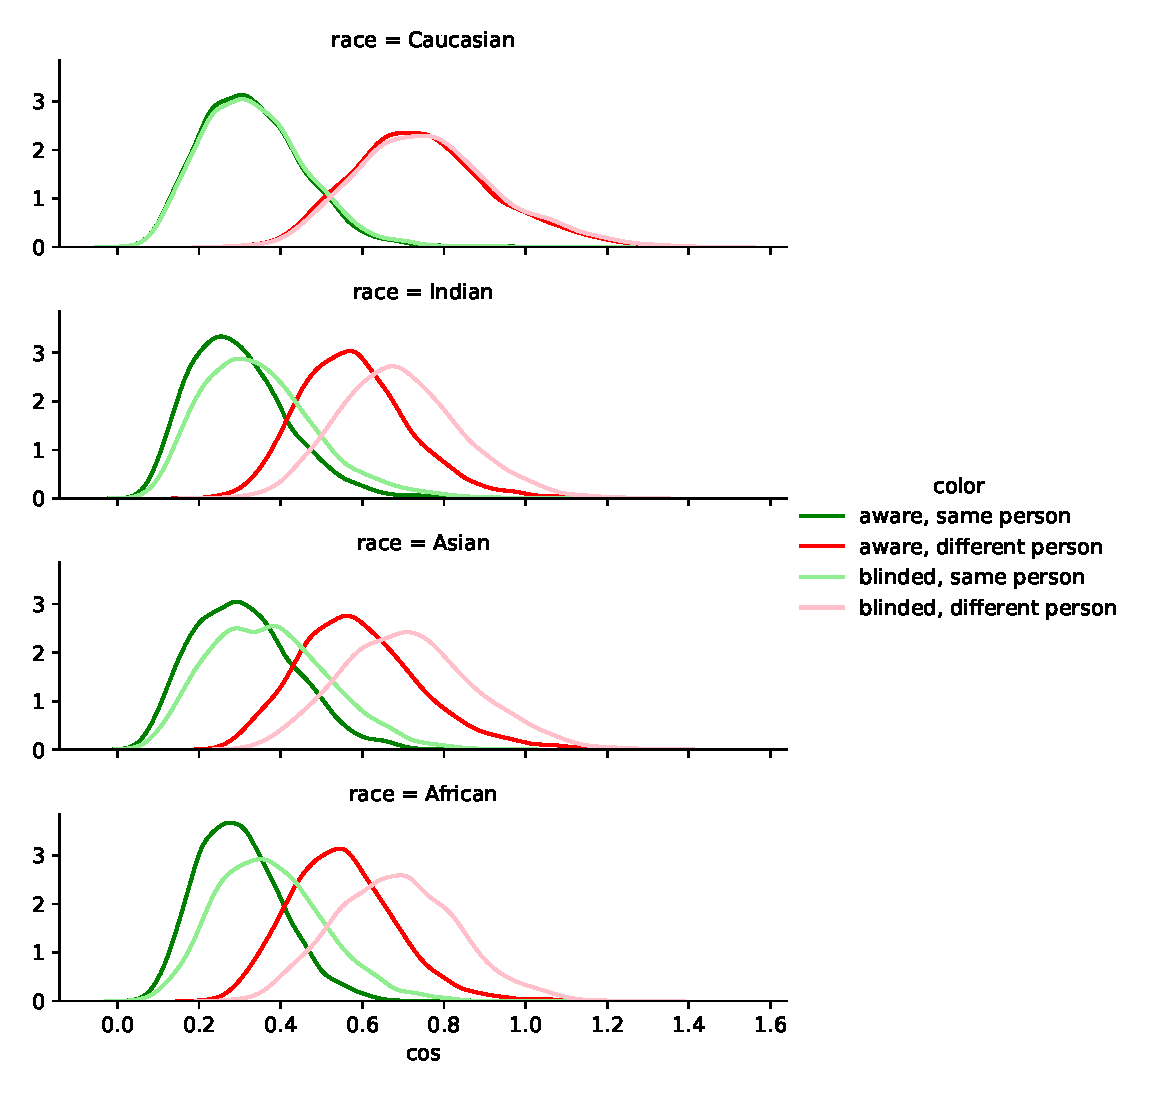
\includegraphics[width=\textwidth]{bias.eps}
  \caption{Kernel density estimation (KDE) plot of pairwise cosine distances for same persons (green) and different persons (red).}
  \label{fig:frrate}
\end{figure}

\section{Discussion}

Most of the findings with regard to the blinding procedures are not surprising. The proposed procedure removes linear separability with the effect that linear classifiers can't distinguish between ethnic clusters after blinding in line with the cluster scores. The fact that the ethnic clusters are well separated in the first place shows that the considered model clearly distinguishes the ethnic groups. The blinding removes some of this information. The surprise comes at the end. The removal of this information actually improves overall performance - but does not remove the bias. The performance improve through this simple linear approach is very surprising. A reason might be that there are a substantial differences between the data used for training of the model and the RFW data used for present benchmark. At this stage it is not clear, whether this performance improve is accidental or generalizes to other models and other discriminatory dimensions.


\end{document}